    \section{Modelo monomial: $V = A|\phi|^n$}
        \label{sec:monomial}

        Implementado en \texttt{models/genmonomial.h}; los \texttt{.in} son \texttt{genmonomial.in} ($n = 6$, exploratorio) y \texttt{genmonomial\_cuartico.in} (el control cuártico de la Sec.~\ref{sec:control}). Para este potencial $A_{\text{eff}} = A$ en el marco común (Sec.~\ref{sec:marco}).

        \subsection{Derivadas}

        \subsection{Derivadas}

            Consideremos que los potenciales monomiales generales para el potencial son de la forma
            \begin{equation}
                V(\phi) = A \left| \phi \right|^n
            \end{equation}
            El valor absoluto es necesario para que $V$ esté bien definido en $\phi < 0$ cuando $n$ no es un entero par.

            Para la implementación de estos modelos en \CosmoLattice debemos calcular sus derivadas primera y segunda:
            \begin{equation}
                V^\prime (\phi) = A n \operatorname{sgn}(\phi) \left| \phi \right|^{n - 1} = A n \, \phi \left| \phi \right|^{n - 2}
            \end{equation}
            \begin{equation}
                V^{\prime \prime} (\phi) = A n (n - 1) \left| \phi \right|^{n - 2}
            \end{equation}
            (para $n < 2$ ambas divergen en $\phi = 0$, y la expresión $\phi |\phi|^{n-2}$ del código da $0 \cdot \infty$ en ese punto).

        \subsection{Variables de programa}

            Con $A_{\text{eff}} = A$ (Sec.~\ref{sec:variables}): $\omega_* = \sqrt{nA}\,\phi_0^{n/2-1}$, $q = g^2\phi_0^{4-n}/(nA)$ y $\tilde V = |\tilde\phi|^n/n + \tfrac12 q\tilde\phi^2\tilde\chi^2$ exactamente (no sólo cerca del mínimo). Con $n = 4$ y $A = \lambda/4$ es \texttt{lphi4}.

        \subsection{Condiciones iniciales y momento inicial}

            Planteemos la condición inicial del campo como aquella tal que $\epsilon = 1$.
            \begin{equation*}
                \begin{split}
                    \epsilon &= \frac{m_p^2}{2} \left[ \frac{V^\prime (\phi)}{V(\phi)} \right]^2\\
                    1 &= \frac{m_p^2}{2} \left[ \frac{V^\prime (\phi_0)}{V(\phi_0)} \right]^2\\
                    \frac{2}{m_p^2} &= \left[ \frac{A n \phi^{n-1}_0}{A \phi^n_0} \right]^2\\
                    \frac{\sqrt{2}}{m_p} &= \frac{n}{\phi_0}\\
                    \phi_0 &= \frac{n}{\sqrt{2}} m_p
                \end{split}
            \end{equation*}
            \begin{equation}
                \phi_0 = \frac{\sqrt{2}}{2} n m_p
            \end{equation}
            Con la fórmula de la Sec.~\ref{sec:momento-inicial} y los parámetros de \texttt{genmonomial.in} ($n = 6$), $\dot\phi_0 = -3.063 \times 10^{31}\,\text{GeV}^2$. Integrando el fondo exacto, $\epsilon_H = 1$ se alcanza en $\phi = 9.04 \times 10^{18}\,\text{GeV}$, contra $\phi_0 = 1.033 \times 10^{19}\,\text{GeV}$.

        \subsection{Ejemplo de inestabilidad con $n = 6$}

            Con las cotas de la Sec.~\ref{sec:estabilidad}, para $n = 6$ ($\alpha = 3/2$), con $N = 64$, $\tilde k_{\text{IR}} = 3$, $\delta\tilde t = 10^{-3}$ y $q = 10^2$, las cotas dan $a_{\max}^{\text{grad}} \simeq 357$ y $a_{\max}^{\text{hijo}} \sim 1170$. En la simulación, la corrida explota en $a \simeq 290$ ($\tilde t \simeq 27$), del orden de la cota del gradiente; por eso \texttt{genmonomial.in} usa $\tilde t_{\max} = 20$ ($a \simeq 190$). Con los parámetros originales ($q = 4 \times 10^4$, $\delta\tilde t = 5 \times 10^{-3}$) la corrida explotaba ya en $\tilde t \simeq 0.5$.

        \subsection{El monomial de control}
            \label{sec:control}

            \texttt{genmonomial\_cuartico.in} \textbf{no es un modelo del paper}: $\lambda\phi^4/4$ como modelo de inflación predice $n_s = 1 - 3/(N_*+1) = 0.946$ y $r = 16/(N_*+1) = 0.29$ para $N_* = 55$ (slow-roll, con $\phi_*^2 = 8(N_*+1)\,m_p^2$), y la cota $r < 0.036$ lo excluye. Lo incluimos para separar qué parte de la señal viene del plateau de los $\alpha$-attractors:
            \begin{itemize}
                \item Usa el $\lambda_{\text{eff}} = 4A_T/M_T^4 = 1.333 \times 10^{-11}$ del T-model, con $A = \lambda_{\text{eff}}/4$. Así, cerca del mínimo tiene el mismo potencial físico que el T-model. Con el mismo $q$ tiene además el mismo acople físico, $g = \sqrt{q\lambda_{\text{eff}}}$, y el mismo $\omega_*/f_*$.
                \item La condición inicial es la de las Secs.~\ref{sec:ci}--\ref{sec:momento-inicial} ($\epsilon_V = 1$): $\phi_0 = 2\sqrt 2\, m_p$. Es mayor que la del T-model, porque sin plateau el slow-roll termina más arriba. En variables de programa los dos arrancan en $\tilde\phi = 1$, pero el monomial lo hace con más energía y más expansión inicial ($a'/a = 0.92$ contra $0.44$).
                \item Es idéntico a \texttt{lphi4} con $\lambda = \lambda_{\text{eff}}$ (Sec.~\ref{sec:variables}), así que también sirve como puente con la comparación con Dufaux \emph{et al.}\ de la Sec.~\ref{sec:literatura}.
            \end{itemize}
            Con $N = 32$ la resonancia llega antes que en el T-model: el campo hijo satura en $\tilde t \simeq 80$, contra $110$ en el T-model, y $\rho_{GW}/\rho$ alcanza el $90\%$ de su valor final en $\tilde t \simeq 230$. El valor final es $2.3 \times 10^{-5}$, contra $1.8 \times 10^{-5}$ en el T-model con la misma $N$. Hay dos cosas a tener en cuenta:
            \begin{itemize}
                \item Como $a'/a(0) = 0.92 > \tilde k_{\text{IR}} = 0.7$, los modos más IR arrancan fuera del horizonte (al final $k_{\text{IR}}/(aH) = 343$). Por lo tanto no conviene bajar $\tilde k_{\text{IR}}$ por debajo de $\sim 0.35$ en este caso.
                \item Con $N = 32$ la cola UV del inflatón es $\sim 10^{-3}$, peor que en los T/E-models, así que hay que correrlo con $N \ge 64$.
            \end{itemize}

        \subsection{Resultados con $N = 64$}
            \label{sec:monomial-N64}

            La comparación con los otros casos está en la Sec.~\ref{sec:resultados-N64}; acá van las figuras de la corrida \texttt{genmonomial\_cuartico.in}, que salen de \texttt{code/analisis\_cosmolattice.py} (las cuatro restantes, \texttt{01\_fondo}, \texttt{03\_espectros\_campos}, \texttt{04\_errores} y \texttt{06\_energias}, quedan en \texttt{build\_corridas/<caso>\_N64\_kIR0.7/analisis/}).

            \begin{figure}[H]
                \centering
                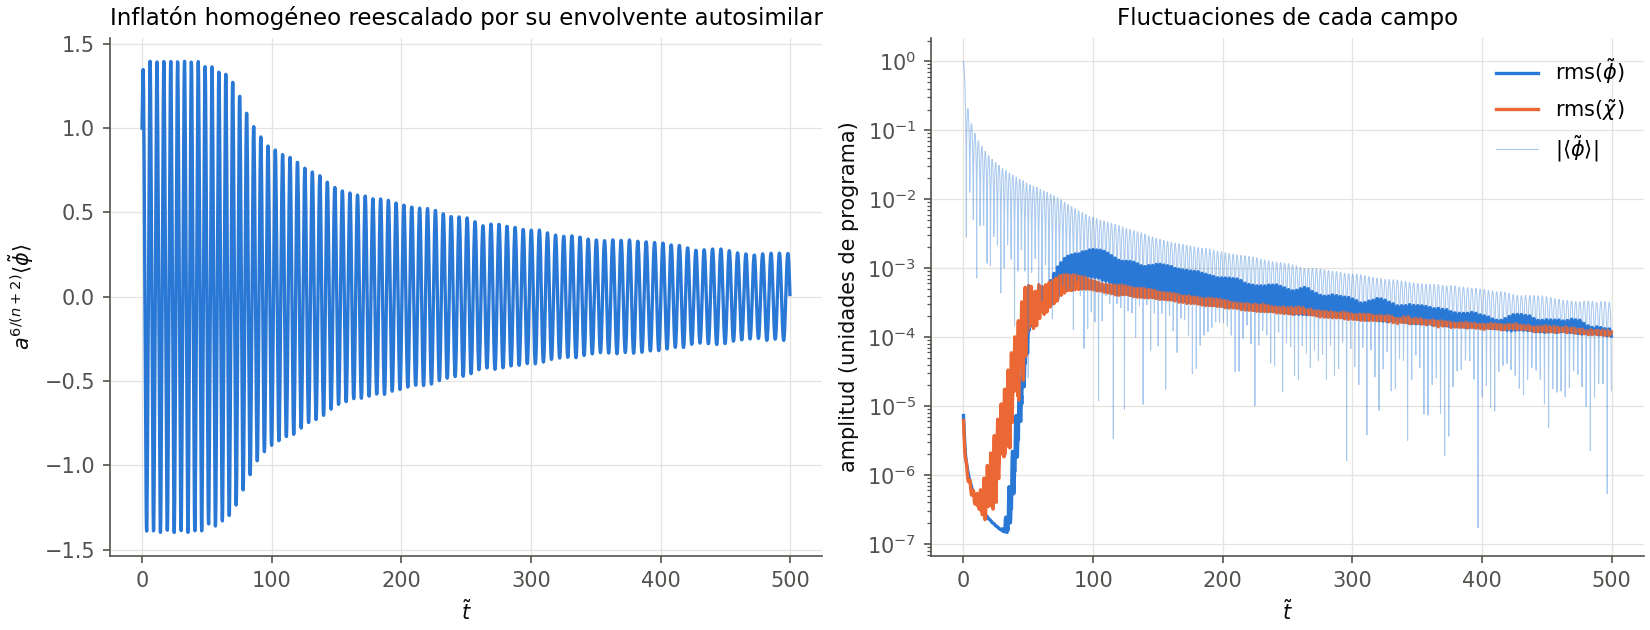
\includegraphics[width=\textwidth]{figuras/genmonomial_cuartico_N64_campos.png}
                \caption{Monomial de control ($\phi^4$), $N = 64$. Izquierda: $\langle\tilde\phi\rangle$ multiplicado por $a^{6/(n+2)} = a$, que sería una oscilación de amplitud constante sin resonancia. Derecha: rms de cada campo y $|\langle\tilde\phi\rangle|$.}
                \label{fig:genmonomial_cuartico-campos}
            \end{figure}
            \begin{figure}[H]
                \centering
                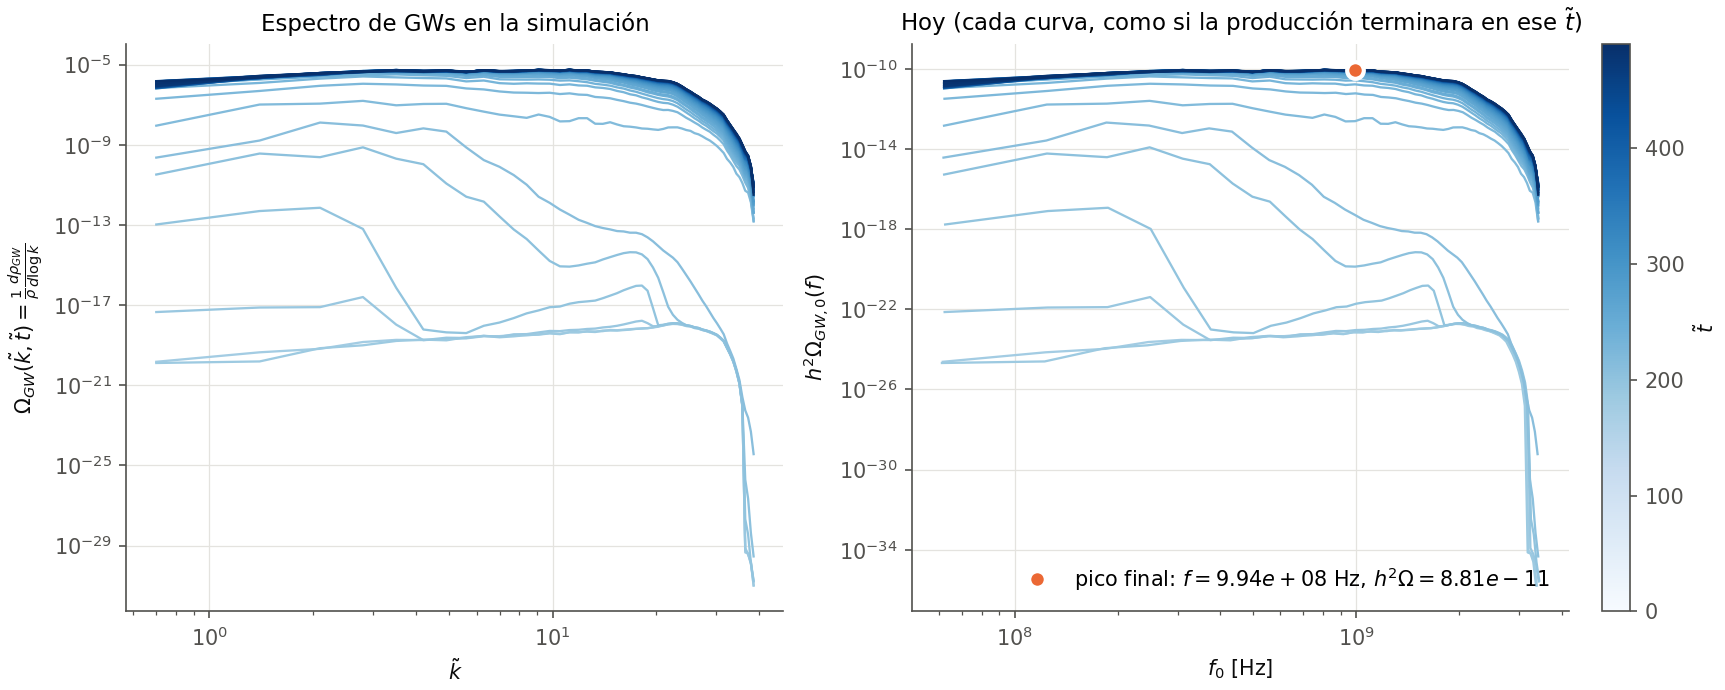
\includegraphics[width=\textwidth]{figuras/genmonomial_cuartico_N64_gws.png}
                \caption{Monomial de control ($\phi^4$), $N = 64$. Espectro de GWs en la red (izquierda) y llevado a hoy (derecha), a cada tiempo de salida (claro = temprano).}
                \label{fig:genmonomial_cuartico-gws}
            \end{figure}

            Con $N = 64$ se confirma lo que se vio con $N = 32$ (Sec.~\ref{sec:control}): sin plateau la resonancia llega antes que en cualquier $\alpha$-attractor. El rms del campo hijo es máximo en $\tilde t = 80$ (T-model: 121), y $\rho_{GW}/\rho$ llega al $90\%$ de su valor final en $\tilde t = 230$. Antes de la resonancia, $\langle\tilde\phi\rangle a$ oscila con amplitud $\simeq 1.4$ (Fig.~\ref{fig:genmonomial_cuartico-campos}), mayor que en el T-model. Es la amplitud que corresponde a arrancar con más energía cinética ($a'/a = 0.92$ contra $0.44$).

            El valor final es $\rho_{GW}/\rho = 1.36 \times 10^{-5}$, contra $2.3 \times 10^{-5}$ con $N = 32$: baja un $40\%$, igual que en el T-model. Es el caso con más potencia UV: el espectro supera la mitad del máximo de $\tilde k = 2.1$ a $17$, y por eso el máximo cae en $\tilde k = 11.2$ (Fig.~\ref{fig:genmonomial_cuartico-gws}). Como el espectro es casi plano en esa banda, la posición del máximo no es robusta (Sec.~\ref{sec:resultados-N64}). Hoy da $h^2\Omega_{GW,0} = 8.8 \times 10^{-11}$ en $9.9 \times 10^8$\,Hz, con más de la mitad del máximo entre $1.9 \times 10^8$ y $1.5 \times 10^9$\,Hz. Es la misma banda que el T-model, aunque el monomial tiene más potencia en $\tilde k$ alto, porque su factor de reescaleo es $1.34$ veces menor. La cola UV de las GWs es $6 \times 10^{-7}$ del máximo, la peor de los cuatro casos pero todavía chica; con $N = 32$ la del inflatón era $\sim 10^{-3}$.

        \subsection{Corridas cuadráticas con $N = 64$}
            \label{sec:monomial-cuadratico}

            La comparación de los cuatro casos cuadráticos (misma grilla, mismo $q$ y misma semilla) y sus limitaciones (el UV no está resuelto y la producción no terminó del todo) están en la Sec.~\ref{sec:resultados-cuadraticos}. Acá van las figuras de \texttt{genmonomial\_cuadratico.in}.

            \begin{figure}[H]
                \centering
                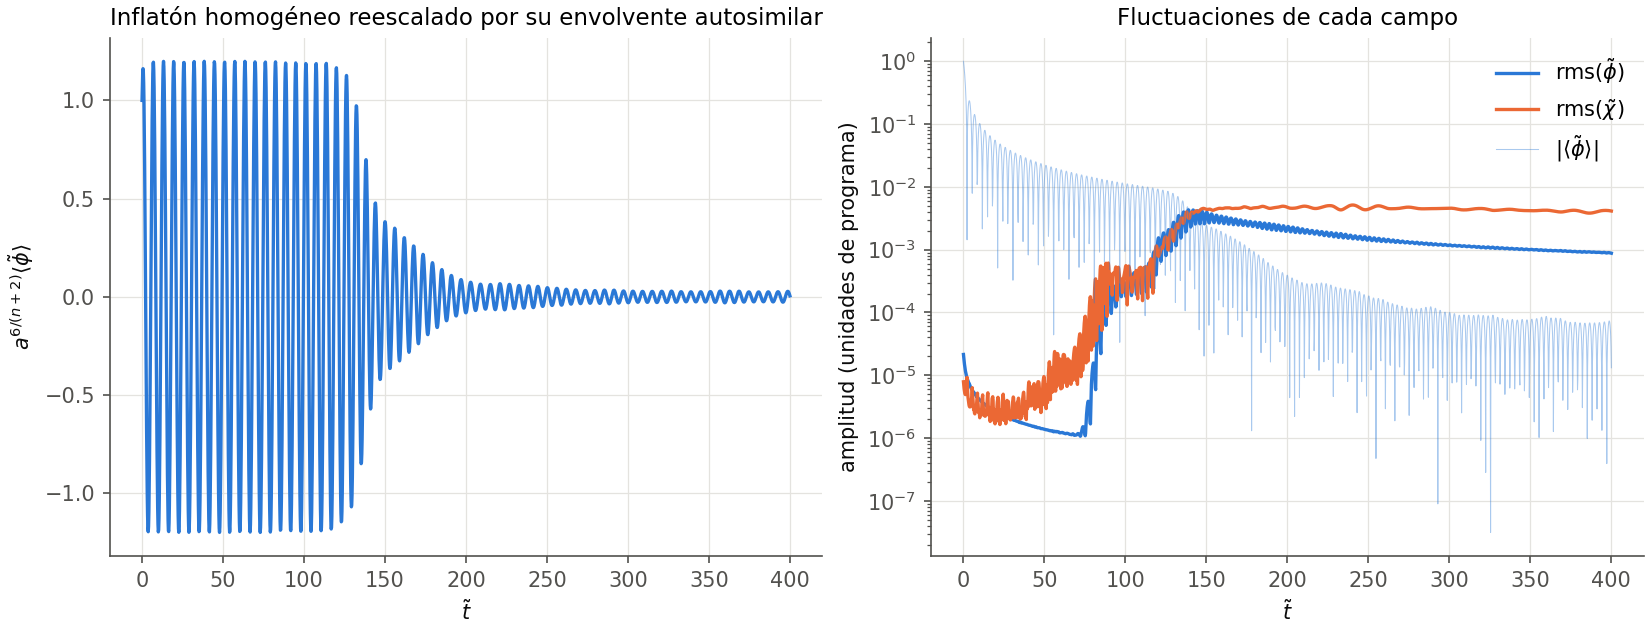
\includegraphics[width=\textwidth]{figuras/genmonomial_cuadratico_N64_campos.png}
                \caption{Monomial cuadrático de control ($m^2\phi^2/2$), $N = 64$. Izquierda: $\langle\tilde\phi\rangle$ multiplicado por $a^{6/(n+2)} = a^{3/2}$, que sin resonancia oscilaría con amplitud constante. Derecha: rms de cada campo y $|\langle\tilde\phi\rangle|$.}
                \label{fig:genmonomial_cuadratico-campos}
            \end{figure}
            \begin{figure}[H]
                \centering
                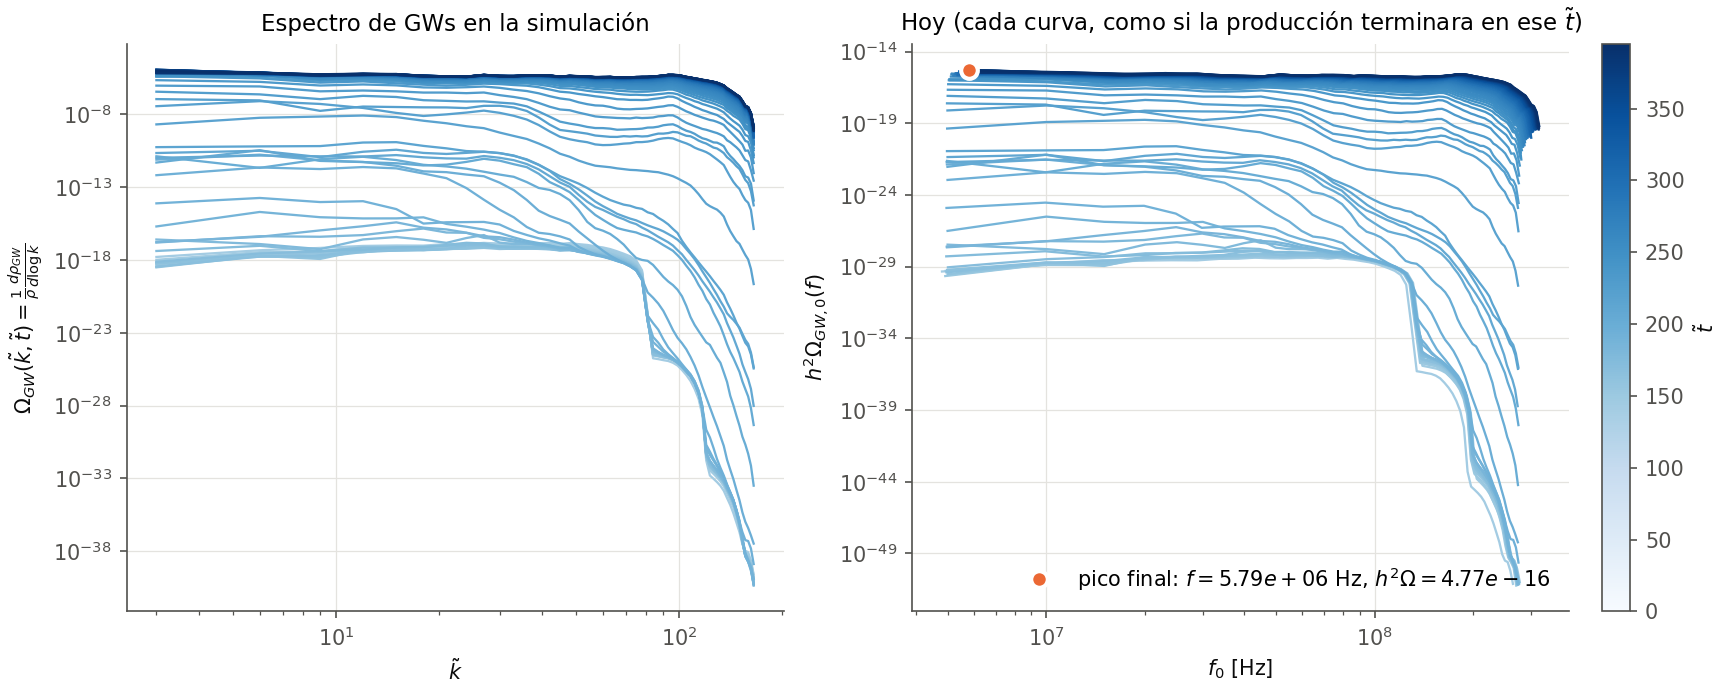
\includegraphics[width=\textwidth]{figuras/genmonomial_cuadratico_N64_gws.png}
                \caption{Monomial cuadrático de control ($m^2\phi^2/2$), $N = 64$. Espectro de GWs en la red (izquierda) y llevado a hoy con $T_{\text{RH}} = 10^{10}$\,GeV y $w = 0$ hasta el reheating (derecha), a cada tiempo de salida (claro = temprano).}
                \label{fig:genmonomial_cuadratico-gws}
            \end{figure}

            \texttt{genmonomial\_cuadratico.in} es $V = m^2\phi^2/2$ con la masa del T-model cuadrático ($\alpha_K = 1$), así que cerca del mínimo tiene el mismo potencial de programa. Está excluido por $r$ ($r = 0.15$ con $N_* = 51.8$). Arranca en $\phi_0 = \sqrt 2\,m_p$, con $a^{3/2}\langle\tilde\phi\rangle$ oscilando con amplitud $\simeq 1.2$, contra $1.09$ en el T-model (Fig.~\ref{fig:genmonomial_cuadratico-campos}).

            Al revés que en el caso cuártico (Sec.~\ref{sec:monomial-N64}), el monomial es el último en resonar: las GWs empiezan a crecer en $\tilde t \simeq 120$, contra $70$--$75$ en los $\alpha$-attractors, y la amplitud del condensado cae a la mitad en $\tilde t \simeq 140$ (T-model: 108). Aun así, es el que más GWs produce: $\rho_{GW}/\rho = 2.46 \times 10^{-5}$, el doble que el T-model, y el más saturado (crece un $4\%$ en los últimos 100 de $\tilde t$). Además tiene más potencia en el IR: $\Omega_{GW,e} \simeq 0.9 \times 10^{-5}$ en $\tilde k = 3$, contra $1.4 \times 10^{-6}$ en el T-model. Como todas las corridas parten de la misma realización de las fluctuaciones, la diferencia viene del potencial; lo que no sabemos, con una sola semilla, es cuánto cambiaría con otra realización.

            Hoy, con $T_{\text{RH}} = 10^{10}$\,GeV y $w = 0$, el máximo es $h^2\Omega_{GW,0} = 4.8 \times 10^{-16}$ en el primer bin ($5.8 \times 10^6$\,Hz), y más de la mitad del máximo cae hasta $1.9 \times 10^8$\,Hz (Fig.~\ref{fig:genmonomial_cuadratico-gws}). Con $\epsilon = 1$ daría $1.5 \times 10^{-10}$ en $1.4 \times 10^8$\,Hz.
